\documentclass[10pt]{article}
\usepackage[utf8]{inputenc}
\usepackage[frenchb]{babel}
\usepackage[T1]{fontenc}
\usepackage{graphics}

\title{Projet 1 Ocaml : Angry Balls}
\date{\today}
\author{Antoine Dailly et Clément Moutet}


\begin{document}

\maketitle

\tableofcontents

\section*{Introduction}


Afin d'évaluer nos compétences en Ocaml, un exercice à la fois rigoureux et intéressant s'imposait. C'est pourquoi il a semblé utile de donner comme exercice aux étudiants suivant le cours de Projet une simulation d'Anrgy Birds.
\par Notre binôme s'est immédiatement attelé à la tâche, avec rigueur et sérieux, afin de fournir un projet suffisamment complet pour être évalué positivement.
\par Ce rapport servira aux correcteurs à évaluer nos choix et notre implémentation du code.
\par Il a été décidé assez vite de modéliser Angry Birds par un jeu de billard avec une gravité : le but du jeu est alors de projeter des boules indestructibles sur des boules cassables afin de les briser.
\par Nous commencerons par expliquer les fonctions gérant les boules de façon interne, avant d'aborder la structure des quadtrees et le problème du déplacement, et enfin nous nous étendrons sur l'interface graphique et utilisateur.


\section{La gestion interne du billard}


\subsection{Boules et collisions}
\subsubsection{Le type 'boule'}
Il a fallu commencer par définir le type boule en Ocaml. Nous avions commencé par simplement la définir par un couple de coordonnées 
représentant son centre (les coordonnées \texttt{x} et \texttt{y}), le rayon \texttt{rayonBoules} ayant été déclaré comme variable globale. Il nous a ensuite été nécessaire d'ajouter des paramètres 
définissant la vitesse (\texttt{vitesseX} et \texttt{vitesseY}), le temps de déplacement relatif (\texttt{tempsDernierDeplacementX} 
et \texttt{tempsDernierDeplacementY}, ainsi que ses paramètres de destructibilité (\texttt{destructibleoupas} et 
\texttt{coefficient\_destruction}).
\par Chacun de ces paramètres sert dans différentes fonctions : si la position permet de dessiner les boules, la vitesse est 
essentielle pour les faire se déplacer et entrer en collision, tandis que le temps de déplacement autorise des trajectoires fluides.
Quant aux paramètres de destructibilité, ils servent à rendre le jeu jouable.
\subsubsection{Collisions avec les bandes}
Afin de rendre le jeu plus amusant, nous avons fait le choix de laisser des bandes. Les retirer serait très simple et finalement moins
divertissant. Le jeu est donc un Angry Birds avec des murs en caoutchouc.
\par La collision avec les bandes, gérée par la fonction \texttt{collisionAvecBandes}, est très simple : quand la boule arrive sur les bandes, on inverse sa vitesse tout en lui soustrayant
le coefficient de frottement. Cela permet de simuler un rebond tout en diminuant la vitesse de la boule.
\subsubsection{Les collisions entre boules}
Les collisions entre boules sont gérées par des appels successifs à la fonction \texttt{gereurDeCollisionsDuneBoule}. Cette fonction va
assurer une grande partie des interactions essentielles entre les boules mises en jeu. Elle prend en argument une boule, et teste si
celle-ci est en collision avec une des autres boules mises en jeu. Si c'est le cas, elle va appliquer plusieurs modifications.
\par Tout d'abord, la fonction va fragilier, voire détruire les boules mises en jeu. À moins que la boule testée ne soit un missile
(et donc indestructible), elle va subir un choc et être fragilisée.
\par Ensuite, elle va modifier la vitesse des deux boules entrées en collision, de manière à les faire rebondir l'une sur l'autre.
\par Ainsi, en appelant successivement cette fonction sur toutes les boules mises en jeu, on pourra gérer leurs collisions !
\subsubsection{Collision de deux boules}
Dans le paragraphe précédent, nous évoquions le test de collision de deux boules entre elles. Voilà comment le test en question a été mis en place :
\par Tout d'abord, par le biais de la fonction \texttt{deux\_Boules\_A\_Cote}, on vérifie si les deux boules sont en contact. Rien de bien compliqué ici.
\par Ensuite, grâce à la fonction \texttt{deux\_boules\_seloignent}, on vérifie si les deux boules s'éloignent ou non, de façon assez simple :
On teste d'abord laquelle est à gauche, puis laquelle est au-dessus, et on finit par vérifier si leurs vitesses respectives les dirigent l'une vers l'autre.
\par Une fois ceci fait, on se contente de tester si les deux boules prises en argument sont côte à côte, et si elles vont l'une vers l'autre.
Cette façon de tester les vitesses permet d'éviter un bug qui nous arrivait souvent : deux boules s'empilant l'une sur l'autre et restant 'collées' l'une à l'autre à cause d'une collision perpétuelle.
On applique ensuite un algorythme connu, trouvé sur Wikipédia, de collision élastique entre deux boules de même masse.

\begin{figure}
 \centering
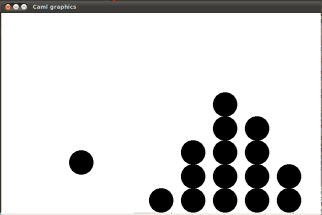
\includegraphics{rapport1.png}
\caption{La disposition initiale}
\end{figure}

\subsection{Gravité et frottements}
\subsubsection{La gravité}
La gravité n'était pas un problème très complexe à mettre en œuvre. Le principe est simple : tant que les boules peuvent être soumises à
la gravité (ie : si elles sont en l'air), on les fait obliquer vers le sol en décroissant le paramètre \texttt{vitesseY}.
\par La fonction auxiliaire \texttt{bouleEstSurUneAutreBoule} détecte si la boule testée est au niveau du sol ou bien si elle est
en équilibre sur une des autres boules mises en jeu. Si c'est pas le cas, on n'applique pas la gravité. Les boules tomberont quand même car la boule du dessous est, elle, toujours soumise à la gravité.
\subsubsection{Les frottements}
Il y a deux types de frottements dans ce jeu : les frottements dûs à l'air et le raclement des boules sur le sol.
\par La fonction \texttt{frottements} applique à chaque boule en mouvement une diminution de leur vitesse, afin de simuler les frottements
de l'air.
\par La fonction \texttt{raclementDeSol} s'applique aux boules qui roulent sur le sol : elle les fait ralentir peu à peu en diminuant
leur vitesse par la constante de frottement statique.
\par Ces deux fonctions sont extrêmement utiles, permettant de simuler plus efficacement les lois physiques qui régissent le billard.


\section{Les quadtrees et le déplacement}


\subsection{Les quadtrees}
\subsubsection{Le type 'quadtree'}
Le type quadtree est un type important dans la modélisation de systèmes physiques dotés d'objets intéragissant au contact les uns des
autres : il permet de s'épargner des calculs inutiles, et donc de fluidifier l'affichage graphique dans ce cas précis.
\par Ce type est défini inductivement de manière très simple : il s'agit en fait d'un arbre quaternaire. Chaque rectangle de la fenêtre
graphique sera divisé en quatre rectangles, et ainsi de suite. De cette manière, les calculs seront fortement simplifiés, car l'ordinateur
n'aura pas à vérifier que deux boules trop éloignées sur la surface de jeu ne sont pas en collision !
\par Qui plus est, le type quadtree contient une liste de boules : il s'agit bien sûr des boules qui se trouvent dans le quadtree concerné.
\subsubsection{La construction des quadtrees}
Il y a deux grandes fonctions intervenant dans la construction des quadtrees : 
\par La fonction \texttt{boulesDansNoeud} qui prend en argument la liste des boules et 4 paramètres correspondant à un rectangle placé sur le terrain : une position x, une position y, une largeur x, et une largeur y. Cette fonction va vérifier pour chaque boule si une partie est dans le rectangle séléctionné, et va renvoyer la liste des boules sur ce rectangle.
\par La fonction \texttt{construireArbreSub}, récursive, qui prend en argument un rectangle, défini par les mêmes paramètres que \texttt{boulesDansNoeud}, et une liste de boules, va diviser le rectangle donné en 4 sous retangles, qu'elle placera dans un quadtree, et y répartir les boules à l'aide de \texttt{boulesDansNoeud}. La fonction va se rapeller sur chacun des sous rectangles, afin de les rediviser, jusqu'à la condition d'arrêt, qui est une largeur x ou une largeur y du rectangle inférieure à rayon + 1. Cette condition d'arrêt à étée choisie car on est sur qu'avec des rectangles de cette taille toutes les collisions possibles seront gérées, ou que soient placées les boules dans le rectangle.

\begin{figure}
 \centering
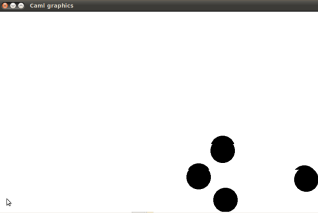
\includegraphics{rapport2.png}
\caption{Les boules se déplaçant}
\end{figure}

\subsection{Le déplacement des boules}
\subsubsection{Les fonctions d'avancée}
Le principe du déplacement adopté est le suivant : on veut faire avancer les boules pixel par pixel, afin de fluidifier le plus possible le mouvement.
\par Pour cela, il nous faut avoir trois fonctions importantes : deux qui feront se déplacer une boule sur un pixel, à l'horizontale ou à la verticale,
et une qui gérera le temps : les boules plus rapides se déplaceront, en toute logique, plus vite que les lentes...
\par Les deux premières fonctions sont \texttt{avancerUnPixelX} et \texttt{avancerUnPixelY}. Elles se contentent de déplacer la boule
passée en argument sans se poser d'autre question.
\par La troisième fonction est en réalité les deux paramètres \texttt{tempsDernierDeplacementX} et \texttt{tempsDernierDeplacementY}.
Ces deux paramètres, indépendants pour chaque boule, sont liés à la vitesse de celle-ci et permettent de faire se déplacer relativement
des boules ayant des vitesses différentes sans difficultés, grâce à la fonction qui sera exposée juste après.
\subsubsection{Le géreur de déplacements}
La fonction \texttt{gereurDeDeplacements} est la fonction principale gérant les mouvements des boules. Elle opère de façon très simple,
en appelant les fonctions définies précédemment.
\par La fonction utilise les paramètres de \texttt{tempsDernierDeplacement (X et Y)} pour gérer les différences de vitesse entre les boules.
Tant que la boule doit encore se déplacer, on la fait avancer grâce aux fonctions \texttt{avancerUnPixel (X et Y)}.
\par Cette méthode de déplacement a l'avantage de rendre l'affichage extrêmement fluide, mais l'inconvénient est qu'elle génère
un très grand nombre de calculs. Pour y pallier, la structure quadtree est particulièrement adaptée.
\par C'est pourquoi la fonction \texttt{deplacementAPartirDarbre} est utilisée pour simplifier les calculs. Le principe est simple : on
coupe l'écran en autant de quadtrees que possible, avant d'effectuer les calculs de déplacement sur chaque unité élémentaire ainsi
obtenue. Cela permet de diminuer le nombre de calculs, et donc de fluidifier l'affichage.
\subsubsection{La fonction bougerBoules}
Cette fonction est véritablement la fonction centrale du programme, celle qui coordonne toutes les fonctions internes de façon cohérente
afin de simuler le jeu de billard. Son fonctionnement est très simple : tant qu'une boule bouge (ceci est calculé via une fonction très
simple, \texttt{uneBouleBouge}), on effectue successivement des fonctions qui vont faire se déplacer les boules de façon réaliste et amusante.
\par On commence par modifier la liste des boules en jeu en supprimant celles qui ont été détruites lors du dernier déplacement à l'aide
d'une fonction auxiliaire, \texttt{supprime\_boules\_detruites} (cette modification de la liste de boules en jeu explique et justifie
l'emploi de références dans cette fonction). Ensuite, on calcule les collisions avec les bandes, puis on applique la gravité, les frottements
au sol ; et enfin on lance la fonction \texttt{deplacementAPartirDarbre}, qui permet de gérer collisions et déplacements.
\par Les derniers effets de la fonction \texttt{bougerBoules} concernent l'affichage graphique, et seront explicités plus tard.
\par Ainsi, cette fonction constitue le cœur de cette simulation. Cependant, le choix de modélisation étant lourd en calculs, il aurait
sans doute été possible de l'optimiser avec un peu plus de temps devant nous.


\section{L'interface graphique et utilisateur}


\subsection{L'interface principale}
\subsubsection{L'affichage des boules}
La fonction \texttt{afficher\_boules} est une fonction assez simple, qui trace des cercles représentant les boules mises en jeu et les peint en noir. À l'origine,
nous avions mis un test qui vérifiait qu'elles ne s'intersectaient pas, mais ce test est devenu inutile vu que les fonctions ne permettent pas qu'une telle
situation arrive.
\par Dans la fonction \texttt{bougerBoules}, le graphique est effacé et les boules sont réaffichéées à chaque déplacement. La fonction
\texttt{afficher\_boules} est à la base de l'interface graphique, car elle permet de visualiser les calculs effectués par l'ordinateur.
\subsubsection{La fonction interface\_utilisateur}
Cette fonction est très clairement la fonction centrale de l'interface. Prenant en argument le nombre de vies choisies par l'utilisateur,
la liste des boules en jeu, elle permet de mettre en branle des fonctions à la fois d'affichage et de fonctionnement 'caché'.
\par Elle commence par assigner une référence, celle de la liste des boules en jeu (on verra plus bas comment cette liste est générée initialement).
Puis, tant que l'utilisateur a encore droit à un essai et tant qu'il restera des boules en jeu, elle effectuera une série d'opérations
visant à mettre en branle le jeu.
\par La fonction va commencer par placer en tête de la liste des boules en jeu le missile que l'utilisateur pourra projeter. Ce missile
se différencie des boules normales par le fait que son paramètre \texttt{destructibleoupas} soit égal à 0 : il est indestructible. Par
la suite, il affiche les boules en jeu. Puis, il appelle la fonction \texttt{force\_et\_direction\_de\_frappe}, qui sera décrite plus tard,
pour laisser le joueur lancer le missile. À partir de là, la machine est lancée : la fonction \texttt{bougerBoules} est appliquée, afin
d'appliquer les déplacements initiés par le joueur. Une fois les déplacements terminés, la fonction s'occupe de nettoyer un peu l'écran,
supprimant les dernières boules détruites et retirant le missile du jeu, avant de descendre le nombre d'essais de l'utilisateur d'un, et
de vérifier si il a remporté la partie ou non (ie : si il reste encore des boules en jeu ou pas).

\begin{figure}
 \centering
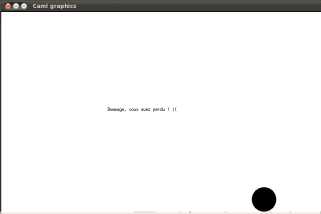
\includegraphics{rapport3.png}
\caption{Dommage...}
\end{figure}

\subsection{Les choix de l'utilisateur}
\subsubsection{Les choix de difficulté}
L'intérêt d'un choix de la difficulté saute aux yeux : chacun peut apprécier le jeu quel que soit son niveau. Dans notre projet, la sélection
de la difficulté s'effectue en deux étapes. Tout d'abord, l'utilisateur est amené à choisir son nombre de missiles (grâce à la fonction \texttt{choix\_nombre\_boules}). Ensuite, il doit choisir
son niveau de difficulté parmi les cinq proposés (grâce à la fonction \texttt{choix\_difficulte}). Plus la difficulté est élevée, plus le joueur aura de boules à détruire, et plus celles-ci
seront résistantes !
\par La fonction \texttt{boules\_selon\_difficulte}, certes peu lisible mais au fond très simple, permet la génération de tours de
boules. Une des améliorations possibles avec plus de temps aurait été de faire des reliefs afin de rendre le jeu plus palpitant et la
fonction de génération des boules moins inintéressante. Mais le manque de temps et de libertés permises par le module graphique d'Ocaml
nous ont forcés à opter pour une solution simple et satisfaisante, bien que peu palpitante.
\subsubsection{Le lancer de boule}
Le principal intérêt d'Angry Birds, c'est de pouvoir jeter une boule sur les autres ! C'est le but de la fonction \texttt{force\_et\_direction\_de\_frappe}
\par Cette fonction utilisele type \texttt{event}, natif du module graphique d'Ocaml, et qui permet d'interpréter certains événements
déclenchés par l'utilisateur : enclenchement ou relâchement de la souris, par exemple.
\par Ici, on attend que le joueur clique sur un missile (si il clique ailleurs, un message d'erreur s'affiche et le système repart dans l'attente
d'un clic). Quand c'est fait, on enregistre la position à laquelle il relâche le bouton, et on en déduit la vitesse imprimée au projectile.

\subsection{Pour finir : le corps principal}
Le corps principal du code permet d'exécuter le programme et de profiter du jeu. Il est ici assez conséquent, mais très simple :
\par On commence par demander au joueur de rentrer, via le terminal, le nombre de vies et la difficulté qu'il souhaite (en appelant les fonctions explicitées dans le paragraphe sur le choix de la difficulté). Ensuite, on ouvre le graphique,
et on appelle les fonctions générant les boules à détruire, et enfin on lance l'\texttt{interface\_utilisateur} avec les paramètres correspondants.
\par Une fois que cette fonction a fini de s'exécuter, c'est à dire une fois que l'utilisateur a lancé tous ses missiles ou qu'il a
détruit toutes les boules, le code attend sagement que le joueur clique, pour fermer le programme.



\section*{Conclusion}


L'implémentation de ce petit jeu en Ocaml nous aura permis de perfectionner notre maîtrise de ce langage, et l'ampleur du projet nous
aura clairement fait coopérer efficacement, tant sur le partage des tâches que sur l'aide et l'apprentissage. De plus, il nous aura
permis d'apprendre à gérer notre temps tout en nous faisant mesurer les difficultés de se coordonner et de concilier efficacité algorithmique
et programmatique.
\par Ce projet nous aura donc clairement fait progresser, et fait mesurer de près les difficultés pouvant surgir lors d'un projet programmation.
\par Dans l'ensemble, nous sommes plutôt contents de notre implémentation : le jeu est fluide et se joue instinctivement tout en laissant
quelques choix cruciaux à l'utilisateur. Ses principales limites sont la lourdeur de certains calculs (notamment ceux occasionnés par notre
choix du déplacement pixel par pixel, qui nous confère une grande fluidité graphiqué ; et par le fait que cette méthode pousse Ocaml dans ses
retranchements, occasionnant par là-même des erreurs d'arrondis), et le peu de variété du jeu étant donné que la disposition sera toujours identique.
Un autre aspect intéressant à améliorer aurait pu être les graphiques, qui sont très simplistes, mais c'est un détail absolument facultatif.
\par En résumé, ce projet fut intéressant à mener et nous a posés des problèmes assez techniques, mais nous avons réussi à le mener à bien,
même si quelques semaines supplémentaires nous auraient permis de le peaufiner.
 



\end{document}
